% Options for packages loaded elsewhere
\PassOptionsToPackage{unicode}{hyperref}
\PassOptionsToPackage{hyphens}{url}
%
\documentclass[
]{article}
\usepackage{amsmath,amssymb}
\usepackage{lmodern}
\usepackage{ifxetex,ifluatex}
\ifnum 0\ifxetex 1\fi\ifluatex 1\fi=0 % if pdftex
  \usepackage[T1]{fontenc}
  \usepackage[utf8]{inputenc}
  \usepackage{textcomp} % provide euro and other symbols
\else % if luatex or xetex
  \usepackage{unicode-math}
  \defaultfontfeatures{Scale=MatchLowercase}
  \defaultfontfeatures[\rmfamily]{Ligatures=TeX,Scale=1}
\fi
% Use upquote if available, for straight quotes in verbatim environments
\IfFileExists{upquote.sty}{\usepackage{upquote}}{}
\IfFileExists{microtype.sty}{% use microtype if available
  \usepackage[]{microtype}
  \UseMicrotypeSet[protrusion]{basicmath} % disable protrusion for tt fonts
}{}
\makeatletter
\@ifundefined{KOMAClassName}{% if non-KOMA class
  \IfFileExists{parskip.sty}{%
    \usepackage{parskip}
  }{% else
    \setlength{\parindent}{0pt}
    \setlength{\parskip}{6pt plus 2pt minus 1pt}}
}{% if KOMA class
  \KOMAoptions{parskip=half}}
\makeatother
\usepackage{xcolor}
\IfFileExists{xurl.sty}{\usepackage{xurl}}{} % add URL line breaks if available
\IfFileExists{bookmark.sty}{\usepackage{bookmark}}{\usepackage{hyperref}}
\hypersetup{
  pdftitle={MUSA 508 Intro to SF},
  pdfauthor={Matt Harris},
  hidelinks,
  pdfcreator={LaTeX via pandoc}}
\urlstyle{same} % disable monospaced font for URLs
\usepackage[margin=1in]{geometry}
\usepackage{color}
\usepackage{fancyvrb}
\newcommand{\VerbBar}{|}
\newcommand{\VERB}{\Verb[commandchars=\\\{\}]}
\DefineVerbatimEnvironment{Highlighting}{Verbatim}{commandchars=\\\{\}}
% Add ',fontsize=\small' for more characters per line
\usepackage{framed}
\definecolor{shadecolor}{RGB}{248,248,248}
\newenvironment{Shaded}{\begin{snugshade}}{\end{snugshade}}
\newcommand{\AlertTok}[1]{\textcolor[rgb]{0.94,0.16,0.16}{#1}}
\newcommand{\AnnotationTok}[1]{\textcolor[rgb]{0.56,0.35,0.01}{\textbf{\textit{#1}}}}
\newcommand{\AttributeTok}[1]{\textcolor[rgb]{0.77,0.63,0.00}{#1}}
\newcommand{\BaseNTok}[1]{\textcolor[rgb]{0.00,0.00,0.81}{#1}}
\newcommand{\BuiltInTok}[1]{#1}
\newcommand{\CharTok}[1]{\textcolor[rgb]{0.31,0.60,0.02}{#1}}
\newcommand{\CommentTok}[1]{\textcolor[rgb]{0.56,0.35,0.01}{\textit{#1}}}
\newcommand{\CommentVarTok}[1]{\textcolor[rgb]{0.56,0.35,0.01}{\textbf{\textit{#1}}}}
\newcommand{\ConstantTok}[1]{\textcolor[rgb]{0.00,0.00,0.00}{#1}}
\newcommand{\ControlFlowTok}[1]{\textcolor[rgb]{0.13,0.29,0.53}{\textbf{#1}}}
\newcommand{\DataTypeTok}[1]{\textcolor[rgb]{0.13,0.29,0.53}{#1}}
\newcommand{\DecValTok}[1]{\textcolor[rgb]{0.00,0.00,0.81}{#1}}
\newcommand{\DocumentationTok}[1]{\textcolor[rgb]{0.56,0.35,0.01}{\textbf{\textit{#1}}}}
\newcommand{\ErrorTok}[1]{\textcolor[rgb]{0.64,0.00,0.00}{\textbf{#1}}}
\newcommand{\ExtensionTok}[1]{#1}
\newcommand{\FloatTok}[1]{\textcolor[rgb]{0.00,0.00,0.81}{#1}}
\newcommand{\FunctionTok}[1]{\textcolor[rgb]{0.00,0.00,0.00}{#1}}
\newcommand{\ImportTok}[1]{#1}
\newcommand{\InformationTok}[1]{\textcolor[rgb]{0.56,0.35,0.01}{\textbf{\textit{#1}}}}
\newcommand{\KeywordTok}[1]{\textcolor[rgb]{0.13,0.29,0.53}{\textbf{#1}}}
\newcommand{\NormalTok}[1]{#1}
\newcommand{\OperatorTok}[1]{\textcolor[rgb]{0.81,0.36,0.00}{\textbf{#1}}}
\newcommand{\OtherTok}[1]{\textcolor[rgb]{0.56,0.35,0.01}{#1}}
\newcommand{\PreprocessorTok}[1]{\textcolor[rgb]{0.56,0.35,0.01}{\textit{#1}}}
\newcommand{\RegionMarkerTok}[1]{#1}
\newcommand{\SpecialCharTok}[1]{\textcolor[rgb]{0.00,0.00,0.00}{#1}}
\newcommand{\SpecialStringTok}[1]{\textcolor[rgb]{0.31,0.60,0.02}{#1}}
\newcommand{\StringTok}[1]{\textcolor[rgb]{0.31,0.60,0.02}{#1}}
\newcommand{\VariableTok}[1]{\textcolor[rgb]{0.00,0.00,0.00}{#1}}
\newcommand{\VerbatimStringTok}[1]{\textcolor[rgb]{0.31,0.60,0.02}{#1}}
\newcommand{\WarningTok}[1]{\textcolor[rgb]{0.56,0.35,0.01}{\textbf{\textit{#1}}}}
\usepackage{graphicx}
\makeatletter
\def\maxwidth{\ifdim\Gin@nat@width>\linewidth\linewidth\else\Gin@nat@width\fi}
\def\maxheight{\ifdim\Gin@nat@height>\textheight\textheight\else\Gin@nat@height\fi}
\makeatother
% Scale images if necessary, so that they will not overflow the page
% margins by default, and it is still possible to overwrite the defaults
% using explicit options in \includegraphics[width, height, ...]{}
\setkeys{Gin}{width=\maxwidth,height=\maxheight,keepaspectratio}
% Set default figure placement to htbp
\makeatletter
\def\fps@figure{htbp}
\makeatother
\setlength{\emergencystretch}{3em} % prevent overfull lines
\providecommand{\tightlist}{%
  \setlength{\itemsep}{0pt}\setlength{\parskip}{0pt}}
\setcounter{secnumdepth}{-\maxdimen} % remove section numbering
\ifluatex
  \usepackage{selnolig}  % disable illegal ligatures
\fi

\title{MUSA 508 Intro to SF}
\author{Matt Harris}
\date{MUSA 508, Fall, 2021}

\begin{document}
\maketitle

{
\setcounter{tocdepth}{2}
\tableofcontents
}
\hypertarget{introduction-to-sf}{%
\subsection{Introduction to SF}\label{introduction-to-sf}}

This markdown document is a gentle introduction to the \texttt{\{sf\}}
package. The intent is not to be exhaustive, but to demonstrate:

\begin{itemize}
\tightlist
\item
  How using \texttt{\{sf\}} allows us to do typical GIS operations
  within R
\item
  Specific aspects of \texttt{\{sf\}} that are used often in the MUSA
  508 assignments
\end{itemize}

Other fantastic resources include:

\begin{itemize}
\tightlist
\item
  The
  \href{https://urbanspatial.github.io/PublicPolicyAnalytics/TOD.html\#setup}{TOD
  Intro} from the course text (Public Policy Analytics)
\item
  The \href{https://r-spatial.github.io/sf/index.html}{`sf' package
  documentation}
\item
  Kyle Walker's \{tidycensus\}
  \href{https://walker-data.com/tidycensus/articles/spatial-data.html}{documentation
  on spatial}
\item
  and many other intro to \texttt{\{sf\}} that are out there.
\end{itemize}

This exercise will pick up where the Week 1 \texttt{\{tidycensus\}} left
off; loading census data using \texttt{geometry\ =\ TRUE} to result in
an \texttt{\{sf\}} object.

\hypertarget{package-setup}{%
\subsection{Package Setup}\label{package-setup}}

\begin{Shaded}
\begin{Highlighting}[]
\FunctionTok{library}\NormalTok{(tidyverse)}
\FunctionTok{library}\NormalTok{(tidycensus)}
\FunctionTok{library}\NormalTok{(sf)}
\FunctionTok{library}\NormalTok{(tmap) }\CommentTok{\# mapping, install if you don\textquotesingle{}t have it}
\FunctionTok{set.seed}\NormalTok{(}\DecValTok{717}\NormalTok{)}
\end{Highlighting}
\end{Shaded}

Your Census API key should be loaded from the week 1 exercise. If you
get an API error about the key, go back and look at the Week 1 markdown.

\hypertarget{recap-get-acs-data-using-tidycensus}{%
\subsection{\texorpdfstring{Recap: Get ACS Data using
\texttt{\{tidycensus\}}}{Recap: Get ACS Data using \{tidycensus\}}}\label{recap-get-acs-data-using-tidycensus}}

We will use the same ACS variables as in the last exercise. The object
called \texttt{acs\_vars} is used to keep the variables we are
interested in. Also, we will focus on specific tracts in the Mt. Airy
neighborhood. Finally, we fetch the data using the \texttt{get\_acs()}
function. The code below is the same code used at the end of Week \#1
with the exception of removing the last line calling
\texttt{st\_as\_af()} . We'll discuss why later.

\begin{Shaded}
\begin{Highlighting}[]
\NormalTok{acs\_vars }\OtherTok{\textless{}{-}} \FunctionTok{c}\NormalTok{(}\StringTok{"B01001\_001E"}\NormalTok{, }\CommentTok{\# ACS total Pop estimate}
              \StringTok{"B25002\_001E"}\NormalTok{, }\CommentTok{\# Estimate of total housing units}
              \StringTok{"B25002\_003E"}\NormalTok{, }\CommentTok{\# Number of vacant housing units}
              \StringTok{"B19013\_001E"}\NormalTok{, }\CommentTok{\# Median HH Income ($)}
              \StringTok{"B02001\_002E"}\NormalTok{, }\CommentTok{\# People describing themselves as "white alone"}
              \StringTok{"B06009\_006E"}\NormalTok{) }\CommentTok{\# Total graduate or professional degree}

\NormalTok{myTracts }\OtherTok{\textless{}{-}} \FunctionTok{c}\NormalTok{(}\StringTok{"42101023500"}\NormalTok{, }
              \StringTok{"42101023600"}\NormalTok{, }
              \StringTok{"42101023700"}\NormalTok{, }
              \StringTok{"42101025300"}\NormalTok{, }
              \StringTok{"42101025400"}\NormalTok{,}
              \StringTok{"42101025500"}\NormalTok{, }
              \StringTok{"42101025600"}\NormalTok{, }
              \StringTok{"42101038800"}\NormalTok{)}

\NormalTok{acsTractsPHL.}\FloatTok{2016.}\NormalTok{sf }\OtherTok{\textless{}{-}} \FunctionTok{get\_acs}\NormalTok{(}\AttributeTok{geography =} \StringTok{"tract"}\NormalTok{,}
                             \AttributeTok{year =} \DecValTok{2016}\NormalTok{, }
                             \AttributeTok{variables =}\NormalTok{ acs\_vars, }
                             \AttributeTok{geometry =} \ConstantTok{TRUE}\NormalTok{, }
                             \AttributeTok{state =} \StringTok{"PA"}\NormalTok{, }
                             \AttributeTok{county =} \StringTok{"Philadelphia"}\NormalTok{, }
                             \AttributeTok{output =} \StringTok{"wide"}\NormalTok{) }\SpecialCharTok{\%\textgreater{}\%} 
\NormalTok{  dplyr}\SpecialCharTok{::}\FunctionTok{select}\NormalTok{ (GEOID, NAME, }\FunctionTok{all\_of}\NormalTok{(acs\_vars)) }\SpecialCharTok{\%\textgreater{}\%}
  \FunctionTok{rename}\NormalTok{ (}\AttributeTok{total\_pop.2016 =}\NormalTok{ B01001\_001E,}
          \AttributeTok{total\_HU.2016 =}\NormalTok{ B25002\_001E,}
          \AttributeTok{total\_vacant.2016 =}\NormalTok{ B25002\_003E,}
          \AttributeTok{med\_HH\_Income.2016 =}\NormalTok{ B19013\_001E,}
          \AttributeTok{total\_White.2016 =}\NormalTok{ B02001\_002E,}
          \AttributeTok{total\_GradDeg.2016 =}\NormalTok{ B06009\_006E) }\SpecialCharTok{\%\textgreater{}\%}
  \FunctionTok{mutate}\NormalTok{(}\AttributeTok{vacancyPct.2016 =}\NormalTok{ total\_vacant}\FloatTok{.2016}\SpecialCharTok{/}\NormalTok{total\_HU}\FloatTok{.2016}\NormalTok{,}
         \AttributeTok{pctWhite.2016 =}\NormalTok{ total\_White}\FloatTok{.2016}\SpecialCharTok{/}\NormalTok{total\_pop}\FloatTok{.2016}\NormalTok{) }\SpecialCharTok{\%\textgreater{}\%}
  \FunctionTok{mutate}\NormalTok{(}\AttributeTok{mtAiry =} \FunctionTok{ifelse}\NormalTok{(GEOID }\SpecialCharTok{\%in\%}\NormalTok{ myTracts, }\StringTok{"MT AIRY"}\NormalTok{, }\StringTok{"REST OF PHILADELPHIA"}\NormalTok{))}
\end{Highlighting}
\end{Shaded}

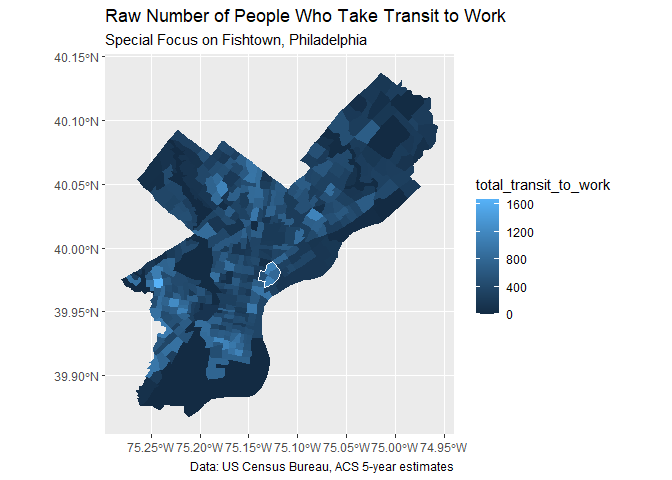
\includegraphics{MUSA_508_Lab2_sf_files/figure-latex/ggplot_geom_sf-1.pdf}

\hypertarget{sf-and-why-spatial-is-special}{%
\subsection{\texorpdfstring{\texttt{\{sf\}} and why spatial is
special}{\{sf\} and why spatial is special}}\label{sf-and-why-spatial-is-special}}

There are two important additions in the above code that allow us to go
from tabular data to spatial data. This is incredibly powerful because
once data has a spatial component, it opens up a whole new world (pun
intended!) of analytical possibilities. Instead of only analyzing how
the variables are correlated, we can now measure how they are correlated
over space, how near, how far, how clustered or dispersed. We have
access to analyzing the entire spatial system that led to these data
being what they are. To quote the Tobler's First Law of Geography,
``\emph{everything is related to everything else, but near things are
more related than distant things.}''
\href{https://en.wikipedia.org/wiki/Tobler\%27s_first_law_of_geography}{wikipedia}.
The rest of this semester will be using spatial relations to better
understand data for more effective public policy.

To understand how the \texttt{\{sf\}} helps us do that, we will break it
down using the \texttt{acsTractsPHL.2016.sf} object we just created from
\texttt{\{tidycensus\}}. Compared to fetching tabular data, the one new
addition to that code is:

\begin{itemize}
\tightlist
\item
  the \texttt{geometry\ =\ TRUE} argument in the call to
  \texttt{get\_acs()}
\end{itemize}

\hypertarget{returning-geometry}{%
\subsubsection{Returning geometry}\label{returning-geometry}}

Using the \texttt{geometry\ =\ TRUE} argument in the \texttt{get\_acs()}
function does a lot of work for us. That argument tells the
\texttt{\{sf\}} package to call on the \texttt{\{tigris\}} package to
download a spatial data (think about a shapefile) from the U.S.
\href{https://www.census.gov/geographies/mapping-files/time-series/geo/tiger-line-file.html}{Tiger/Line}
for the level of detail requested (e.g.~state, county, tract,
etc\ldots), join the tabular ACS data to the geometry using the
\texttt{GEOID} field, and then turn it into an \texttt{\{sf\}} object
that R can use to map and analyze. Looking into the
\texttt{acsTractsPHL.2016.sf} object, we can understand this better.

\begin{Shaded}
\begin{Highlighting}[]
\FunctionTok{class}\NormalTok{(acsTractsPHL.}\FloatTok{2016.}\NormalTok{sf)}
\end{Highlighting}
\end{Shaded}

\begin{verbatim}
## [1] "sf"         "data.frame"
\end{verbatim}

First, we can see what \texttt{class} the \texttt{acsTractsPHL.2016.sf}
object is. It is class \texttt{sf} first and then \texttt{data.frame}
second. This means that you can write R code to treat this as a spatial
class, but that you can also do a lot of the things you would normally
do with a \texttt{data.frame} to it as well. That is very handy!

If we print the \texttt{acsTractsPHL.2016.sf} object, it looks a lot
like a table, but has some extra information at the top that it is an
\texttt{\{sf\}} object and has attributes aside from the tabular data.

\begin{Shaded}
\begin{Highlighting}[]
\FunctionTok{head}\NormalTok{(acsTractsPHL.}\FloatTok{2016.}\NormalTok{sf,}\DecValTok{2}\NormalTok{)}
\end{Highlighting}
\end{Shaded}

\begin{verbatim}
## Simple feature collection with 2 features and 11 fields
## Geometry type: MULTIPOLYGON
## Dimension:     XY
## Bounding box:  xmin: -75.23584 ymin: 39.96507 xmax: -75.22407 ymax: 39.99188
## Geodetic CRS:  NAD83
##         GEOID                                                NAME
## 1 42101010200 Census Tract 102, Philadelphia County, Pennsylvania
## 2 42101011900 Census Tract 119, Philadelphia County, Pennsylvania
##   total_pop.2016 total_HU.2016 total_vacant.2016 med_HH_Income.2016
## 1           3008          1483               225              16071
## 2           4738          2509               407              30854
##   total_White.2016 total_GradDeg.2016                       geometry
## 1                0                145 MULTIPOLYGON (((-75.23536 3...
## 2               47                175 MULTIPOLYGON (((-75.23367 3...
##   vacancyPct.2016 pctWhite.2016               mtAiry
## 1       0.1517195   0.000000000 REST OF PHILADELPHIA
## 2       0.1622160   0.009919797 REST OF PHILADELPHIA
\end{verbatim}

You will notice new information at the top of the print out from the
\texttt{acsTractsPHL.2016.sf\$geometry} object. This includes:

\begin{itemize}
\tightlist
\item
  Simple feature collection with 2 features and 11 fields
\item
  geometry type: MULTIPOLYGON
\item
  dimension: XY
\item
  bbox: xmin: -75.23584 ymin: 39.96507 xmax: -75.22407 ymax: 39.99188
\item
  geographic CRS: NAD83
\end{itemize}

The first line tells you that you have a ``Simple feature'' collection
of a certain number of rows and columns. More on this later, but
\texttt{sf} stands for ``simple features''. We only have 2 features here
because I limited it to two in the code above to save room. The
\texttt{geometry\ type} tell us that the data is represented as a
polygon; an area represented by at least three sides. The could also be
POINT or POLYLINE if there data were represented as points or lines. The
\texttt{dimension} tells us how the data are measured. It will typically
always be ``XY'' in our class. Next the \texttt{bbox} tells us what the
bounding box is for these data. The bounding box is the smallest
rectangle that can be drawn to fit all of the data points. The numbers
tell us the coordinates of the sides of the bbox. From that we can
figure out what the corners are as demonstrated below. The final bit of
information is the \texttt{geographic\ CRS} which stands for coordinate
reference system.

You noticed in the bbox line that the box is measured in some way, in
this case it is familiar latitude and longitude. However, we can measure
geographic space using thousands of different coordinate systems. This
is a major theme in this course; \textbf{There are many different ways
to measure things in space. Each method has trade offs. You will have to
know the basic systems and how to move data between them.} You could
spend an entire career learning about coordinate systems, but for this
course, you will only need the basics. More on that below.

\includegraphics[width=5.28125in,height=\textheight]{IMG/Varying-bounding-box-coordinates-each-bounding-box-is-created-based-on-the-minimum-and.png}

\hypertarget{how-does-sf-store-geometry}{%
\subsubsection{\texorpdfstring{How does \texttt{\{sf\}} store
geometry?}{How does \{sf\} store geometry?}}\label{how-does-sf-store-geometry}}

We just learned that an \texttt{sf} object contains spatial information
in the form of coordinates. In the case of
\texttt{acsTractsPHL.2016.sf}, the coordinates form polygons. To see how
this is stored, we can look at the \texttt{geometry} column.

\begin{Shaded}
\begin{Highlighting}[]
\NormalTok{acsTractsPHL.}\FloatTok{2016.}\NormalTok{sf}\SpecialCharTok{$}\NormalTok{geometry}
\end{Highlighting}
\end{Shaded}

\begin{verbatim}
## Geometry set for 384 features 
## Geometry type: MULTIPOLYGON
## Dimension:     XY
## Bounding box:  xmin: -75.28027 ymin: 39.86705 xmax: -74.95578 ymax: 40.13799
## Geodetic CRS:  NAD83
## First 5 geometries:
\end{verbatim}

\begin{verbatim}
## MULTIPOLYGON (((-75.23536 39.96851, -75.2357 39...
\end{verbatim}

\begin{verbatim}
## MULTIPOLYGON (((-75.23367 39.99188, -75.22566 3...
\end{verbatim}

\begin{verbatim}
## MULTIPOLYGON (((-75.17785 39.97425, -75.17378 3...
\end{verbatim}

\begin{verbatim}
## MULTIPOLYGON (((-75.13877 39.97932, -75.13814 3...
\end{verbatim}

\begin{verbatim}
## MULTIPOLYGON (((-75.13902 39.98876, -75.13835 3...
\end{verbatim}

The \texttt{geometry} column is special column in an \texttt{sf} object
that contains the spatial information. It is stored as plain human
readable text:
\texttt{MULTIPOLYGON\ (((-75.23536\ 39.96851,\ -75.2357\ 39\ldots{}} The
specific format of this text is the
\href{https://r-spatial.github.io/sf/articles/sf1.html}{Simple Features
standard}. This a widely used standard which means there are lots of
resources about it and lots of tools/packages/software that implement
it. It is also where the \texttt{\{sf\}} packages gets its name! In the
example above, the \texttt{geometry} column says that the object is a
Multipart Polygon and then lists out all of the coordinates in longitude
and latitude. For very complex shapes like a coast line you can imagine
that this column could contain millions of coordinates and become quite
large! That will be a consideration during this course so keep it in
mind.

If you look at what class the \texttt{geometry} column is, you can see
that it is a class \texttt{"sfc\_MULTIPOLYGON"\ "sfc"} . This is
different from typical data.frame column classes such as
\texttt{character} or \texttt{numeric}. The \texttt{sfc} in this special
class means \emph{simple features collection}.

\begin{Shaded}
\begin{Highlighting}[]
\FunctionTok{class}\NormalTok{(acsTractsPHL.}\FloatTok{2016.}\NormalTok{sf}\SpecialCharTok{$}\NormalTok{geometry)}
\end{Highlighting}
\end{Shaded}

\begin{verbatim}
## [1] "sfc_MULTIPOLYGON" "sfc"
\end{verbatim}

The \texttt{geometry} column as an \texttt{sfc} can stand on its own, be
plotted and analyzed, but it isn't very interesting without the
associated data. Adding the interesting data is exactly what the
\texttt{geometry\ =\ TRUE} argument of \texttt{get\_acs()} does for us.
Putting it together, \texttt{data.frame} + \texttt{sfc} = \texttt{sf}!

\hypertarget{what-about-the-coordinates}{%
\subsubsection{What about the
Coordinates?}\label{what-about-the-coordinates}}

The rabbit hole of understanding coordinate reference systems is very
deep. We will only go down to the first level, but here are the things
you need to start out with:

\begin{itemize}
\item
  all spatial data need a CRS, otherwise they cannot be measured in
  space and cannot be spatially analyzed.
\item
  you need to know, or figure out, the CRS for all of the spatial data
  you work with. It is not enough just to guess. You will need to figure
  it out through looking at data sources and mapping data to confirm
\item
  There are two main types of CRS, Projected and Unprojected (aka
  Geographic) coordinate systems. Projected Coordinate Systems (PCS) are
  how we map/project the round earth onto a flat map. Common examples of
  PCS are State Plane, UTM, and Mercator coordinate systems. Geographic
  Coordinate Systems (GCS) are how we located things on the round'ish
  earth. Common examples are WGS84, GRS80, and NAD83. Every PCS is based
  on a CGS, but a GCS can be mapped on its own.
\item
  The most common GCS is WGS84, also known as
  \href{https://epsg.io/4326}{\texttt{EPSG:4326}} . This is a very
  common CRS and the default for many mapping applications and mapping
  libraries like \texttt{leaflet} . You will use it very often.
\item
  To measure the distance between things, use a PCS such as State Plane
  or UTM with units in meters or feet. Trying to measure distances in
  Lat/Lon and GCS will often be difficult because the length of a meter
  (or a foot) changes in a GCS as you move north or south from the
  equator. A typical pattern is to project the data into UTM or similar
  for a step in the analysis and then move back to \texttt{4326} for
  mapping and other uses.
\item
  Here are some good places to start on these topics
  \href{https://geocompr.robinlovelace.net/reproj-geo-data.html\#introduction-3}{Geocomputation
  in R},
  \href{https://www.esri.com/arcgis-blog/products/arcgis-pro/mapping/gcs_vs_pcs/}{ESRI
  Geographic vs.~Projected Coordinate Systems}, and
  \href{https://mgimond.github.io/Spatial/chp09_0.html}{Introduction to
  Spatial Analysis in R}
\end{itemize}

Below we will go over some basic ways into interact with the CRS in
\texttt{\{sf\}}.

\hypertarget{manipulating-the-crs-of-an-sf-object}{%
\subsection{\texorpdfstring{Manipulating the CRS of an \texttt{sf}
object}{Manipulating the CRS of an sf object}}\label{manipulating-the-crs-of-an-sf-object}}

We saw that the \texttt{acsTractsPHL.2016.sf} object has a CRS of
\texttt{NAD83} when we inspected it. This CRS was automatically set by
\texttt{\{tidycensus\}} because it knows where the data comes from. This
will not always be the case! A format with a shapefile that has CRS
information in the metadata will likely assign properly, but if you load
a CSV with point coordinates, \texttt{\{sf\}} will not guess as to which
CRS it is. We will see how to assign a CRS soon.

To get a more in depth view of the CRS information in
\texttt{acsTractsPHL.2016.sf} we use the \texttt{st\_csr} function in
\texttt{\{sf\}}.

\emph{Note: the majority of functions you will use in the
\texttt{\{sf\}} package start with the prefix \texttt{st\_}. This is a
convention from spatial databases and used by \texttt{\{sf\}} for
consistency.}

\begin{Shaded}
\begin{Highlighting}[]
\FunctionTok{st\_crs}\NormalTok{(acsTractsPHL.}\FloatTok{2016.}\NormalTok{sf)}
\end{Highlighting}
\end{Shaded}

\begin{verbatim}
## Coordinate Reference System:
##   User input: NAD83 
##   wkt:
## GEOGCRS["NAD83",
##     DATUM["North American Datum 1983",
##         ELLIPSOID["GRS 1980",6378137,298.257222101,
##             LENGTHUNIT["metre",1]]],
##     PRIMEM["Greenwich",0,
##         ANGLEUNIT["degree",0.0174532925199433]],
##     CS[ellipsoidal,2],
##         AXIS["latitude",north,
##             ORDER[1],
##             ANGLEUNIT["degree",0.0174532925199433]],
##         AXIS["longitude",east,
##             ORDER[2],
##             ANGLEUNIT["degree",0.0174532925199433]],
##     ID["EPSG",4269]]
\end{verbatim}

This gives us two bits of info, the CRS as NAD83 and then the CRS in the
\textbf{wkt} format; this stands for well-known-text. The wkt is a human
readable version of the CRS specification with important information.
There are a lot of numbers, but the important to us parts are the
\texttt{GEOGCRS} at the start so we see it is a GCS and
\texttt{ID{[}"EPSG",4269{]}} at the end so we know the EPSG code.

\begin{Shaded}
\begin{Highlighting}[]
\FunctionTok{tm\_shape}\NormalTok{(acsTractsPHL.}\FloatTok{2016.}\NormalTok{sf,}
         \AttributeTok{projection =} \FunctionTok{st\_crs}\NormalTok{(acsTractsPHL.}\FloatTok{2016.}\NormalTok{sf)) }\SpecialCharTok{+}
  \FunctionTok{tm\_fill}\NormalTok{() }\SpecialCharTok{+}
  \FunctionTok{tm\_borders}\NormalTok{() }\SpecialCharTok{+}
  \FunctionTok{tm\_layout}\NormalTok{(}\AttributeTok{title=} \StringTok{\textquotesingle{}NAD83\textquotesingle{}}\NormalTok{, }
            \AttributeTok{title.position =} \FunctionTok{c}\NormalTok{(}\StringTok{\textquotesingle{}left\textquotesingle{}}\NormalTok{, }\StringTok{\textquotesingle{}top\textquotesingle{}}\NormalTok{))}
\end{Highlighting}
\end{Shaded}

\includegraphics{MUSA_508_Lab2_sf_files/figure-latex/unnamed-chunk-6-1.pdf}

\hypertarget{reprojecting-the-crs}{%
\subsubsection{Reprojecting the CRS}\label{reprojecting-the-crs}}

Moving our data into a different projection is usually easy in
\texttt{\{sf\}} with the \texttt{st\_transform()} function. Here we will
re-project our data from the GCS of \texttt{NAD83} to the PCS of
\texttt{UTM\ Zone\ 18N} which stands for the Universal Transverse
Mercator PCS. Specifically the
\href{https://www.spatialreference.org/ref/epsg/wgs-84-utm-zone-18n/}{18
North zone of UTM}. The UTM PCS is a very useful projection!

\includegraphics[width=4.16667in,height=\textheight]{IMG/Utm-zones-USA.svg.png}

\hypertarget{pcs---utm-zone-18-north}{%
\paragraph{PCS - UTM Zone 18 North}\label{pcs---utm-zone-18-north}}

Here is the code to reproject our data.

\begin{Shaded}
\begin{Highlighting}[]
\NormalTok{acsTractsPHL.}\FloatTok{2016.}\NormalTok{sf\_UTM }\OtherTok{\textless{}{-}}\NormalTok{ acsTractsPHL.}\FloatTok{2016.}\NormalTok{sf }\SpecialCharTok{\%\textgreater{}\%} 
  \FunctionTok{st\_transform}\NormalTok{(}\AttributeTok{crs =} \StringTok{"EPSG:26918"}\NormalTok{)}

\FunctionTok{st\_crs}\NormalTok{(acsTractsPHL.}\FloatTok{2016.}\NormalTok{sf\_UTM)}
\end{Highlighting}
\end{Shaded}

\begin{verbatim}
## Coordinate Reference System:
##   User input: EPSG:26918 
##   wkt:
## PROJCRS["NAD83 / UTM zone 18N",
##     BASEGEOGCRS["NAD83",
##         DATUM["North American Datum 1983",
##             ELLIPSOID["GRS 1980",6378137,298.257222101,
##                 LENGTHUNIT["metre",1]]],
##         PRIMEM["Greenwich",0,
##             ANGLEUNIT["degree",0.0174532925199433]],
##         ID["EPSG",4269]],
##     CONVERSION["UTM zone 18N",
##         METHOD["Transverse Mercator",
##             ID["EPSG",9807]],
##         PARAMETER["Latitude of natural origin",0,
##             ANGLEUNIT["degree",0.0174532925199433],
##             ID["EPSG",8801]],
##         PARAMETER["Longitude of natural origin",-75,
##             ANGLEUNIT["degree",0.0174532925199433],
##             ID["EPSG",8802]],
##         PARAMETER["Scale factor at natural origin",0.9996,
##             SCALEUNIT["unity",1],
##             ID["EPSG",8805]],
##         PARAMETER["False easting",500000,
##             LENGTHUNIT["metre",1],
##             ID["EPSG",8806]],
##         PARAMETER["False northing",0,
##             LENGTHUNIT["metre",1],
##             ID["EPSG",8807]]],
##     CS[Cartesian,2],
##         AXIS["(E)",east,
##             ORDER[1],
##             LENGTHUNIT["metre",1]],
##         AXIS["(N)",north,
##             ORDER[2],
##             LENGTHUNIT["metre",1]],
##     USAGE[
##         SCOPE["Engineering survey, topographic mapping."],
##         AREA["North America - between 78°W and 72°W - onshore and offshore. Canada - Nunavut; Ontario; Quebec. United States (USA) - Connecticut; Delaware; Maryland; Massachusetts; New Hampshire; New Jersey; New York; North Carolina; Pennsylvania; Virginia; Vermont."],
##         BBOX[28.28,-78,84,-72]],
##     ID["EPSG",26918]]
\end{verbatim}

We can see the numerous additions to the CRS output including the
\texttt{PROJCRS} title instead of \texttt{GEOGCRS} and all of the
projection parameters that map space to a flat space. Comparing the map
below to the \texttt{NAD83} map shows a little difference in
orientation, but it is not very noticeable. However, in the new
\texttt{UTM83\ 18N} version, you will see that we are in CRS with a set
length unit \texttt{LENGTHUNIT{[}"metre",1{]}} so that we can measure
distance in an accurate way.

\begin{Shaded}
\begin{Highlighting}[]
\FunctionTok{tm\_shape}\NormalTok{(acsTractsPHL.}\FloatTok{2016.}\NormalTok{sf\_UTM, }
         \AttributeTok{projection =} \FunctionTok{st\_crs}\NormalTok{(acsTractsPHL.}\FloatTok{2016.}\NormalTok{sf\_UTM)) }\SpecialCharTok{+}
  \FunctionTok{tm\_fill}\NormalTok{() }\SpecialCharTok{+}
  \FunctionTok{tm\_borders}\NormalTok{() }\SpecialCharTok{+}
  \FunctionTok{tm\_layout}\NormalTok{(}\AttributeTok{title=} \StringTok{\textquotesingle{}UTM 18N\textquotesingle{}}\NormalTok{, }
            \AttributeTok{title.position =} \FunctionTok{c}\NormalTok{(}\StringTok{\textquotesingle{}left\textquotesingle{}}\NormalTok{, }\StringTok{\textquotesingle{}top\textquotesingle{}}\NormalTok{))}
\end{Highlighting}
\end{Shaded}

\includegraphics{MUSA_508_Lab2_sf_files/figure-latex/unnamed-chunk-8-1.pdf}

\hypertarget{pcs---usa-contiguous-albers-equal-area}{%
\paragraph{PCS - USA Contiguous albers equal
area}\label{pcs---usa-contiguous-albers-equal-area}}

UTM is great for local and regional scale data that fit within a single
zone. Sometimes we need data across a broader scale. Also, sometimes was
need a CRS that is not in the EPSG system. Here we use a common ESRI
based projection that has the domain of the continental U.S. Using a
non-EPSG domain is as easy as using \texttt{crs\ =\ "ESRI:102003"}

\begin{Shaded}
\begin{Highlighting}[]
\NormalTok{acsTractsPHL.}\FloatTok{2016.}\NormalTok{sf\_Albers }\OtherTok{\textless{}{-}}\NormalTok{ acsTractsPHL.}\FloatTok{2016.}\NormalTok{sf }\SpecialCharTok{\%\textgreater{}\%} 
  \FunctionTok{st\_transform}\NormalTok{(}\AttributeTok{crs =} \StringTok{"ESRI:102003"}\NormalTok{)}

\FunctionTok{st\_crs}\NormalTok{(acsTractsPHL.}\FloatTok{2016.}\NormalTok{sf\_Albers)}
\end{Highlighting}
\end{Shaded}

\begin{verbatim}
## Coordinate Reference System:
##   User input: ESRI:102003 
##   wkt:
## PROJCRS["USA_Contiguous_Albers_Equal_Area_Conic",
##     BASEGEOGCRS["NAD83",
##         DATUM["North American Datum 1983",
##             ELLIPSOID["GRS 1980",6378137,298.257222101,
##                 LENGTHUNIT["metre",1]]],
##         PRIMEM["Greenwich",0,
##             ANGLEUNIT["Degree",0.0174532925199433]]],
##     CONVERSION["USA_Contiguous_Albers_Equal_Area_Conic",
##         METHOD["Albers Equal Area",
##             ID["EPSG",9822]],
##         PARAMETER["Latitude of false origin",37.5,
##             ANGLEUNIT["Degree",0.0174532925199433],
##             ID["EPSG",8821]],
##         PARAMETER["Longitude of false origin",-96,
##             ANGLEUNIT["Degree",0.0174532925199433],
##             ID["EPSG",8822]],
##         PARAMETER["Latitude of 1st standard parallel",29.5,
##             ANGLEUNIT["Degree",0.0174532925199433],
##             ID["EPSG",8823]],
##         PARAMETER["Latitude of 2nd standard parallel",45.5,
##             ANGLEUNIT["Degree",0.0174532925199433],
##             ID["EPSG",8824]],
##         PARAMETER["Easting at false origin",0,
##             LENGTHUNIT["metre",1],
##             ID["EPSG",8826]],
##         PARAMETER["Northing at false origin",0,
##             LENGTHUNIT["metre",1],
##             ID["EPSG",8827]]],
##     CS[Cartesian,2],
##         AXIS["(E)",east,
##             ORDER[1],
##             LENGTHUNIT["metre",1]],
##         AXIS["(N)",north,
##             ORDER[2],
##             LENGTHUNIT["metre",1]],
##     USAGE[
##         SCOPE["Not known."],
##         AREA["United States (USA) - CONUS onshore - Alabama; Arizona; Arkansas; California; Colorado; Connecticut; Delaware; Florida; Georgia; Idaho; Illinois; Indiana; Iowa; Kansas; Kentucky; Louisiana; Maine; Maryland; Massachusetts; Michigan; Minnesota; Mississippi; Missouri; Montana; Nebraska; Nevada; New Hampshire; New Jersey; New Mexico; New York; North Carolina; North Dakota; Ohio; Oklahoma; Oregon; Pennsylvania; Rhode Island; South Carolina; South Dakota; Tennessee; Texas; Utah; Vermont; Virginia; Washington; West Virginia; Wisconsin; Wyoming."],
##         BBOX[24.41,-124.79,49.38,-66.91]],
##     ID["ESRI",102003]]
\end{verbatim}

Compared to the UTM and NAD83 version, you can see Broad St.~is much
closer to a North/South alignment. This is a pretty good projection for
Philadelphia Data.

\begin{Shaded}
\begin{Highlighting}[]
\FunctionTok{tm\_shape}\NormalTok{(acsTractsPHL.}\FloatTok{2016.}\NormalTok{sf\_Albers, }
         \AttributeTok{projection =} \FunctionTok{st\_crs}\NormalTok{(acsTractsPHL.}\FloatTok{2016.}\NormalTok{sf\_Albers)) }\SpecialCharTok{+}
  \FunctionTok{tm\_fill}\NormalTok{() }\SpecialCharTok{+}
  \FunctionTok{tm\_borders}\NormalTok{() }\SpecialCharTok{+}
  \FunctionTok{tm\_layout}\NormalTok{(}\AttributeTok{title=} \StringTok{\textquotesingle{}USA Contiguous albers\textquotesingle{}}\NormalTok{, }
            \AttributeTok{title.position =} \FunctionTok{c}\NormalTok{(}\StringTok{\textquotesingle{}left\textquotesingle{}}\NormalTok{, }\StringTok{\textquotesingle{}top\textquotesingle{}}\NormalTok{))}
\end{Highlighting}
\end{Shaded}

\includegraphics{MUSA_508_Lab2_sf_files/figure-latex/unnamed-chunk-10-1.pdf}

\hypertarget{gcs---wgs84}{%
\paragraph{GCS - WGS84}\label{gcs---wgs84}}

Finally, we can easily project our data back to a GCS, this time using
the standard \texttt{EPSG:4326} which will allow us to map in many
common frameworks like leaflet.

\begin{Shaded}
\begin{Highlighting}[]
\NormalTok{acsTractsPHL.}\FloatTok{2016.}\NormalTok{sf\_WGS84 }\OtherTok{\textless{}{-}}\NormalTok{ acsTractsPHL.}\FloatTok{2016.}\NormalTok{sf }\SpecialCharTok{\%\textgreater{}\%} 
  \FunctionTok{st\_transform}\NormalTok{(}\AttributeTok{crs =} \StringTok{"EPSG:4326"}\NormalTok{)}

\FunctionTok{st\_crs}\NormalTok{(acsTractsPHL.}\FloatTok{2016.}\NormalTok{sf\_WGS84)}
\end{Highlighting}
\end{Shaded}

\begin{verbatim}
## Coordinate Reference System:
##   User input: EPSG:4326 
##   wkt:
## GEOGCRS["WGS 84",
##     DATUM["World Geodetic System 1984",
##         ELLIPSOID["WGS 84",6378137,298.257223563,
##             LENGTHUNIT["metre",1]]],
##     PRIMEM["Greenwich",0,
##         ANGLEUNIT["degree",0.0174532925199433]],
##     CS[ellipsoidal,2],
##         AXIS["geodetic latitude (Lat)",north,
##             ORDER[1],
##             ANGLEUNIT["degree",0.0174532925199433]],
##         AXIS["geodetic longitude (Lon)",east,
##             ORDER[2],
##             ANGLEUNIT["degree",0.0174532925199433]],
##     USAGE[
##         SCOPE["Horizontal component of 3D system."],
##         AREA["World."],
##         BBOX[-90,-180,90,180]],
##     ID["EPSG",4326]]
\end{verbatim}

\begin{Shaded}
\begin{Highlighting}[]
\FunctionTok{tm\_shape}\NormalTok{(acsTractsPHL.}\FloatTok{2016.}\NormalTok{sf\_WGS84, }
         \AttributeTok{projection =} \FunctionTok{st\_crs}\NormalTok{(acsTractsPHL.}\FloatTok{2016.}\NormalTok{sf\_WGS84)) }\SpecialCharTok{+}
  \FunctionTok{tm\_fill}\NormalTok{() }\SpecialCharTok{+}
  \FunctionTok{tm\_borders}\NormalTok{() }\SpecialCharTok{+}
  \FunctionTok{tm\_layout}\NormalTok{(}\AttributeTok{title=} \StringTok{\textquotesingle{}USA Contiguous albers\textquotesingle{}}\NormalTok{, }
            \AttributeTok{title.position =} \FunctionTok{c}\NormalTok{(}\StringTok{\textquotesingle{}left\textquotesingle{}}\NormalTok{, }\StringTok{\textquotesingle{}top\textquotesingle{}}\NormalTok{))}
\end{Highlighting}
\end{Shaded}

\includegraphics{MUSA_508_Lab2_sf_files/figure-latex/unnamed-chunk-12-1.pdf}

\hypertarget{projecting-new-data}{%
\subsection{Projecting new data}\label{projecting-new-data}}

Often times we are making data or receive data in a format that does not
carry any CRS information. Hopefully, you know what the CRS is or can
ask the person that sent it. If you don't have that you can google your
data source. The last resort is having to try a number of different
projections until your data lines up the way you want it to. This can be
quite a challenge.

Here we will create some data for Philadelphia. This is an example as if
you just read in a CSV file of points.

\begin{Shaded}
\begin{Highlighting}[]
\NormalTok{PHL\_data }\OtherTok{\textless{}{-}} \FunctionTok{data.frame}\NormalTok{(}\AttributeTok{point\_ID =} \FunctionTok{seq}\NormalTok{(}\DecValTok{1}\NormalTok{,}\DecValTok{300}\NormalTok{,}\DecValTok{1}\NormalTok{),}
                       \AttributeTok{variable1 =} \FunctionTok{rnorm}\NormalTok{(}\DecValTok{300}\NormalTok{,}\DecValTok{0}\NormalTok{,}\DecValTok{1}\NormalTok{)) }\SpecialCharTok{\%\textgreater{}\%} 
            \FunctionTok{mutate}\NormalTok{(}\AttributeTok{latitude  =} \FunctionTok{sample}\NormalTok{(}\FunctionTok{seq}\NormalTok{(}\FloatTok{39.852}\NormalTok{,}\FloatTok{40.052}\NormalTok{,}\FloatTok{0.001}\NormalTok{),}\FunctionTok{n}\NormalTok{(), }\AttributeTok{replace =} \ConstantTok{TRUE}\NormalTok{),}
                   \AttributeTok{longitude =} \FunctionTok{sample}\NormalTok{(}\FunctionTok{seq}\NormalTok{(}\SpecialCharTok{{-}}\FloatTok{75.265}\NormalTok{,}\SpecialCharTok{{-}}\FloatTok{75.065}\NormalTok{,}\FloatTok{0.001}\NormalTok{),}\FunctionTok{n}\NormalTok{(), }\AttributeTok{replace =} \ConstantTok{TRUE}\NormalTok{))}

\FunctionTok{head}\NormalTok{(PHL\_data)}
\end{Highlighting}
\end{Shaded}

\begin{verbatim}
##   point_ID  variable1 latitude longitude
## 1        1  1.3982972   39.896   -75.098
## 2        2  0.6425140   39.950   -75.147
## 3        3 -0.1128888   39.970   -75.176
## 4        4 -0.2124540   40.020   -75.218
## 5        5  0.2063796   40.012   -75.129
## 6        6  0.2751510   40.028   -75.135
\end{verbatim}

In this case we will know that the CRS is \texttt{4326}. We can assign
the CRS with the \texttt{st\_as\_af()} function and the \texttt{coords}
argument to specify the columns with longitude and latitude (In that
order!) and the \texttt{crs} argument with the \texttt{"EPSG:4326"}
designation.

\begin{Shaded}
\begin{Highlighting}[]
\NormalTok{PHL\_data.sf }\OtherTok{\textless{}{-}}\NormalTok{ PHL\_data }\SpecialCharTok{\%\textgreater{}\%} 
  \FunctionTok{st\_as\_sf}\NormalTok{(}\AttributeTok{coords =} \FunctionTok{c}\NormalTok{(}\StringTok{"longitude"}\NormalTok{, }\StringTok{"latitude"}\NormalTok{),}
           \AttributeTok{crs =} \StringTok{"EPSG:4326"}\NormalTok{) }
\end{Highlighting}
\end{Shaded}

Combining the points with our ACS tract outlines works since both
objects have the same CRS of \texttt{4326}.

\begin{Shaded}
\begin{Highlighting}[]
\FunctionTok{tm\_shape}\NormalTok{(acsTractsPHL.}\FloatTok{2016.}\NormalTok{sf\_WGS84) }\SpecialCharTok{+}
    \FunctionTok{tm\_borders}\NormalTok{() }\SpecialCharTok{+}
\FunctionTok{tm\_shape}\NormalTok{(PHL\_data.sf) }\SpecialCharTok{+}
    \FunctionTok{tm\_symbols}\NormalTok{(}\AttributeTok{col =} \StringTok{"red"}\NormalTok{) }\SpecialCharTok{+}
\FunctionTok{tm\_legend}\NormalTok{(}\AttributeTok{show =} \ConstantTok{FALSE}\NormalTok{) }\SpecialCharTok{+}
   \FunctionTok{tm\_layout}\NormalTok{(}\AttributeTok{title=} \StringTok{\textquotesingle{}WGS84 {-} 4326\textquotesingle{}}\NormalTok{, }
            \AttributeTok{title.position =} \FunctionTok{c}\NormalTok{(}\StringTok{\textquotesingle{}left\textquotesingle{}}\NormalTok{, }\StringTok{\textquotesingle{}top\textquotesingle{}}\NormalTok{))}
\end{Highlighting}
\end{Shaded}

\includegraphics{MUSA_508_Lab2_sf_files/figure-latex/unnamed-chunk-15-1.pdf}

\hypertarget{extracting-removing-geometry}{%
\subsection{Extracting \& Removing
Geometry}\label{extracting-removing-geometry}}

Finally, another common operation is to remove the geometry to either do
non-spatial analytics or transform in some way and join back to the
data.

\hypertarget{removing-geometry}{%
\subsubsection{Removing geometry}\label{removing-geometry}}

To remove the geometry all together is as easy as using
\texttt{st\_drop\_geometry()}. This leaves you with a plain data.frame
with all aspects of the spatial data removed, including the geometry
column.

\begin{Shaded}
\begin{Highlighting}[]
\NormalTok{acsTractsPHL}\FloatTok{.2016}\NormalTok{\_nonsf }\OtherTok{\textless{}{-}} \FunctionTok{st\_drop\_geometry}\NormalTok{(acsTractsPHL.}\FloatTok{2016.}\NormalTok{sf)}
\end{Highlighting}
\end{Shaded}

\hypertarget{polygon-centroids}{%
\subsubsection{Polygon Centroids}\label{polygon-centroids}}

Another very common thing is to get the
\href{https://geocompr.robinlovelace.net/geometric-operations.html\#centroids}{centroids}
of the polygons.

\begin{Shaded}
\begin{Highlighting}[]
\NormalTok{acsTractsPHL}\FloatTok{.2016}\NormalTok{\_centroid }\OtherTok{\textless{}{-}}\NormalTok{ acsTractsPHL.}\FloatTok{2016.}\NormalTok{sf }\SpecialCharTok{\%\textgreater{}\%} 
  \FunctionTok{st\_centroid}\NormalTok{()}
\end{Highlighting}
\end{Shaded}

\begin{verbatim}
## Warning in st_centroid.sf(.): st_centroid assumes attributes are constant over
## geometries of x
\end{verbatim}

\begin{Shaded}
\begin{Highlighting}[]
\FunctionTok{head}\NormalTok{(acsTractsPHL}\FloatTok{.2016}\NormalTok{\_centroid)}
\end{Highlighting}
\end{Shaded}

\begin{verbatim}
## Simple feature collection with 6 features and 11 fields
## Geometry type: POINT
## Dimension:     XY
## Bounding box:  xmin: -75.23167 ymin: 39.96808 xmax: -75.13394 ymax: 39.9918
## Geodetic CRS:  NAD83
##         GEOID                                                NAME
## 1 42101010200 Census Tract 102, Philadelphia County, Pennsylvania
## 2 42101011900 Census Tract 119, Philadelphia County, Pennsylvania
## 3 42101013900 Census Tract 139, Philadelphia County, Pennsylvania
## 4 42101015700 Census Tract 157, Philadelphia County, Pennsylvania
## 5 42101016300 Census Tract 163, Philadelphia County, Pennsylvania
## 6 42101016800 Census Tract 168, Philadelphia County, Pennsylvania
##   total_pop.2016 total_HU.2016 total_vacant.2016 med_HH_Income.2016
## 1           3008          1483               225              16071
## 2           4738          2509               407              30854
## 3           2960          1342               218              14314
## 4           2688          1128               238              38991
## 5           3710          1252               173              14017
## 6           3605          1940               405              17250
##   total_White.2016 total_GradDeg.2016                   geometry
## 1                0                145 POINT (-75.23167 39.96808)
## 2               47                175 POINT (-75.22881 39.98613)
## 3              466                 74 POINT (-75.17112 39.97499)
## 4             1485                147 POINT (-75.13552 39.97804)
## 5             1605                 10  POINT (-75.13394 39.9885)
## 6              154                 99  POINT (-75.16762 39.9918)
##   vacancyPct.2016 pctWhite.2016               mtAiry
## 1       0.1517195   0.000000000 REST OF PHILADELPHIA
## 2       0.1622160   0.009919797 REST OF PHILADELPHIA
## 3       0.1624441   0.157432432 REST OF PHILADELPHIA
## 4       0.2109929   0.552455357 REST OF PHILADELPHIA
## 5       0.1381789   0.432614555 REST OF PHILADELPHIA
## 6       0.2087629   0.042718447 REST OF PHILADELPHIA
\end{verbatim}

\begin{Shaded}
\begin{Highlighting}[]
\FunctionTok{tm\_shape}\NormalTok{(acsTractsPHL.}\FloatTok{2016.}\NormalTok{sf\_WGS84) }\SpecialCharTok{+}
    \FunctionTok{tm\_borders}\NormalTok{() }\SpecialCharTok{+}
\FunctionTok{tm\_shape}\NormalTok{(acsTractsPHL}\FloatTok{.2016}\NormalTok{\_centroid) }\SpecialCharTok{+}
    \FunctionTok{tm\_symbols}\NormalTok{(}\AttributeTok{col =} \StringTok{"red"}\NormalTok{) }\SpecialCharTok{+}
\FunctionTok{tm\_legend}\NormalTok{(}\AttributeTok{show =} \ConstantTok{FALSE}\NormalTok{) }\SpecialCharTok{+}
   \FunctionTok{tm\_layout}\NormalTok{(}\AttributeTok{title=} \StringTok{\textquotesingle{}Polygon Centroids\textquotesingle{}}\NormalTok{, }
            \AttributeTok{title.position =} \FunctionTok{c}\NormalTok{(}\StringTok{\textquotesingle{}left\textquotesingle{}}\NormalTok{, }\StringTok{\textquotesingle{}top\textquotesingle{}}\NormalTok{))}
\end{Highlighting}
\end{Shaded}

\includegraphics{MUSA_508_Lab2_sf_files/figure-latex/unnamed-chunk-18-1.pdf}

\hypertarget{extracting-geometry}{%
\subsubsection{Extracting Geometry}\label{extracting-geometry}}

Quite often we want a list of the centroid coordinates for analysis of
the coordinates or to join to other data. The \texttt{st\_coordinates()}
function makes that quite easy! Running that on the centroid data leaves
us with a simple data frame of X and Y coordinates.

\begin{Shaded}
\begin{Highlighting}[]
\NormalTok{acsTractsPHL}\FloatTok{.2016}\NormalTok{\_coords }\OtherTok{\textless{}{-}}\NormalTok{ acsTractsPHL}\FloatTok{.2016}\NormalTok{\_centroid }\SpecialCharTok{\%\textgreater{}\%} 
  \FunctionTok{st\_coordinates}\NormalTok{()}

\FunctionTok{head}\NormalTok{(acsTractsPHL}\FloatTok{.2016}\NormalTok{\_coords)}
\end{Highlighting}
\end{Shaded}

\begin{verbatim}
##           X        Y
## 1 -75.23167 39.96808
## 2 -75.22881 39.98613
## 3 -75.17112 39.97499
## 4 -75.13552 39.97804
## 5 -75.13394 39.98850
## 6 -75.16762 39.99180
\end{verbatim}

\hypertarget{binding-geometry}{%
\paragraph{Binding Geometry}\label{binding-geometry}}

Sometimes we need to do operations on tables or non-spatial data where
the geometry column gets in the way. In this case you can sometime drop
the geometry, do what is needed, and then bind it back. A note of
caution here, when you \texttt{cbind()} there are no checks that the
rows of the two data sets are in the same order. They have to be the
same number of rows, but if you analysis resorted or arranged one data
set, the coords of the other will bind, but not be the correct
coordinates. This is why checking your work with plots and maps is
always a good idea!

\begin{Shaded}
\begin{Highlighting}[]
\NormalTok{acsTractsPHL\_Income\_coords }\OtherTok{\textless{}{-}} \FunctionTok{st\_drop\_geometry}\NormalTok{(acsTractsPHL.}\FloatTok{2016.}\NormalTok{sf) }\SpecialCharTok{\%\textgreater{}\%} 
  \FunctionTok{select}\NormalTok{(GEOID, med\_HH\_Income}\FloatTok{.2016}\NormalTok{) }\SpecialCharTok{\%\textgreater{}\%} 
  \FunctionTok{cbind}\NormalTok{(acsTractsPHL}\FloatTok{.2016}\NormalTok{\_coords)}

\FunctionTok{head}\NormalTok{(acsTractsPHL\_Income\_coords)}
\end{Highlighting}
\end{Shaded}

\begin{verbatim}
##         GEOID med_HH_Income.2016         X        Y
## 1 42101010200              16071 -75.23167 39.96808
## 2 42101011900              30854 -75.22881 39.98613
## 3 42101013900              14314 -75.17112 39.97499
## 4 42101015700              38991 -75.13552 39.97804
## 5 42101016300              14017 -75.13394 39.98850
## 6 42101016800              17250 -75.16762 39.99180
\end{verbatim}

A safer way to add the coordinate column and retain it with the index
column \texttt{GEOID} without the fear of accidentally reordering the
rows is to use \texttt{dplyr::mutate} . This assigned the coordinate
columns inline and guarantees that they match.

\begin{Shaded}
\begin{Highlighting}[]
\NormalTok{GEOID\_Coords }\OtherTok{\textless{}{-}}\NormalTok{ acsTractsPHL}\FloatTok{.2016}\NormalTok{\_centroid }\SpecialCharTok{\%\textgreater{}\%}
\NormalTok{  dplyr}\SpecialCharTok{::}\FunctionTok{mutate}\NormalTok{(}\AttributeTok{longitude =}\NormalTok{ sf}\SpecialCharTok{::}\FunctionTok{st\_coordinates}\NormalTok{(.)[,}\DecValTok{1}\NormalTok{],}
                \AttributeTok{latitude =}\NormalTok{ sf}\SpecialCharTok{::}\FunctionTok{st\_coordinates}\NormalTok{(.)[,}\DecValTok{2}\NormalTok{]) }\SpecialCharTok{\%\textgreater{}\%} 
  \FunctionTok{st\_drop\_geometry}\NormalTok{() }\SpecialCharTok{\%\textgreater{}\%} 
  \FunctionTok{select}\NormalTok{(GEOID, latitude, longitude)}

\FunctionTok{head}\NormalTok{(GEOID\_Coords)}
\end{Highlighting}
\end{Shaded}

\begin{verbatim}
##         GEOID latitude longitude
## 1 42101010200 39.96808 -75.23167
## 2 42101011900 39.98613 -75.22881
## 3 42101013900 39.97499 -75.17112
## 4 42101015700 39.97804 -75.13552
## 5 42101016300 39.98850 -75.13394
## 6 42101016800 39.99180 -75.16762
\end{verbatim}

\hypertarget{table-join-with-geometry}{%
\paragraph{Table Join with Geometry}\label{table-join-with-geometry}}

Finally, with the \texttt{GEOID\_Coords} data.frame above, we have
simple table the has our ID column as \texttt{GEOID} and X/Y point
coordinates. This is itself, not an \texttt{sf} object, but it contains
spatial information in coordinate form. WIth this we can make any other
non-spatial table into an \texttt{sf} object as long as it has the
\texttt{GEOID} column.

The example below pretends that \texttt{new\_nonspatial\_data} is some
data we just loaded that has the \texttt{GEOID}, but no additional
spatial information. We go on to further modify that table with a filer
and a sort so that it no longer has the same number of rows or same
order as before. Our approach of using \texttt{cbind} to add the
geometry would fail here. Fortunately, we can use the power of
\href{https://stat545.com/join-cheatsheet.html}{table joins} to help.
Here we use \texttt{left\_join()} to only join the lat/lon coordinates
that match the \texttt{GEOID} in the filtered/sorted table. We specify
to join on the \texttt{GEOID} field with \texttt{by\ =\ "GEOID"}. Then
we use \texttt{st\_as\_sf()} as we had before to make normal table into
an \texttt{sf} object with the correct CRS. Finally, we use
\texttt{st\_transform()} to reproject it to a coordinate system for
mapping with out other data.

\begin{Shaded}
\begin{Highlighting}[]
\NormalTok{new\_nonspatial\_data }\OtherTok{\textless{}{-}} \FunctionTok{st\_drop\_geometry}\NormalTok{(acsTractsPHL.}\FloatTok{2016.}\NormalTok{sf) }

\NormalTok{new\_nonspatial\_data\_filter }\OtherTok{\textless{}{-}}\NormalTok{ new\_nonspatial\_data }\SpecialCharTok{\%\textgreater{}\%} 
  \FunctionTok{filter}\NormalTok{(vacancyPct}\FloatTok{.2016} \SpecialCharTok{\textgreater{}} \FloatTok{0.3}\NormalTok{) }\SpecialCharTok{\%\textgreater{}\%} 
  \FunctionTok{arrange}\NormalTok{(}\FunctionTok{desc}\NormalTok{(med\_HH\_Income}\FloatTok{.2016}\NormalTok{))}

\NormalTok{filter\_data\_joined\_sf }\OtherTok{\textless{}{-}}\NormalTok{ new\_nonspatial\_data\_filter }\SpecialCharTok{\%\textgreater{}\%} 
  \FunctionTok{left\_join}\NormalTok{(GEOID\_Coords, }\AttributeTok{by =} \StringTok{"GEOID"}\NormalTok{) }\SpecialCharTok{\%\textgreater{}\%} 
  \FunctionTok{st\_as\_sf}\NormalTok{(}\AttributeTok{coords =} \FunctionTok{c}\NormalTok{(}\StringTok{"longitude"}\NormalTok{, }\StringTok{"latitude"}\NormalTok{),}
                      \AttributeTok{crs =} \StringTok{"EPSG:4269"}\NormalTok{) }\SpecialCharTok{\%\textgreater{}\%} 
  \FunctionTok{st\_transform}\NormalTok{(}\AttributeTok{crs =} \StringTok{"EPSG:4326"}\NormalTok{)}

\FunctionTok{head}\NormalTok{(filter\_data\_joined\_sf) }
\end{Highlighting}
\end{Shaded}

\begin{verbatim}
## Simple feature collection with 6 features and 11 fields
## Geometry type: POINT
## Dimension:     XY
## Bounding box:  xmin: -75.20931 ymin: 39.9333 xmax: -75.1509 ymax: 40.01119
## Geodetic CRS:  WGS 84
##         GEOID                                                   NAME
## 1 42101012203 Census Tract 122.03, Philadelphia County, Pennsylvania
## 2 42101020102 Census Tract 201.02, Philadelphia County, Pennsylvania
## 3 42101015101 Census Tract 151.01, Philadelphia County, Pennsylvania
## 4 42101003200     Census Tract 32, Philadelphia County, Pennsylvania
## 5 42101020000    Census Tract 200, Philadelphia County, Pennsylvania
## 6 42101016902 Census Tract 169.02, Philadelphia County, Pennsylvania
##   total_pop.2016 total_HU.2016 total_vacant.2016 med_HH_Income.2016
## 1            643           742               384              38438
## 2           3083          1678               531              32066
## 3           2317          1165               388              30051
## 4           4631          2268               709              27256
## 5           1327           766               241              25066
## 6           5797          2912               954              24802
##   total_White.2016 total_GradDeg.2016 vacancyPct.2016 pctWhite.2016
## 1              312                135       0.5175202   0.485225505
## 2                8                 68       0.3164482   0.002594875
## 3               74                 16       0.3330472   0.031937851
## 4              392                109       0.3126102   0.084646945
## 5               50                 85       0.3146214   0.037678975
## 6               88                 68       0.3276099   0.015180266
##                 mtAiry                   geometry
## 1 REST OF PHILADELPHIA POINT (-75.20931 40.00757)
## 2 REST OF PHILADELPHIA POINT (-75.15453 40.01119)
## 3 REST OF PHILADELPHIA POINT (-75.18575 39.98696)
## 4 REST OF PHILADELPHIA  POINT (-75.18542 39.9333)
## 5 REST OF PHILADELPHIA  POINT (-75.1509 40.00253)
## 6 REST OF PHILADELPHIA POINT (-75.18319 39.99398)
\end{verbatim}

\begin{Shaded}
\begin{Highlighting}[]
\FunctionTok{tm\_shape}\NormalTok{(acsTractsPHL.}\FloatTok{2016.}\NormalTok{sf\_WGS84) }\SpecialCharTok{+}
    \FunctionTok{tm\_borders}\NormalTok{() }\SpecialCharTok{+}
\FunctionTok{tm\_shape}\NormalTok{(filter\_data\_joined\_sf) }\SpecialCharTok{+}
    \FunctionTok{tm\_symbols}\NormalTok{(}\AttributeTok{col =} \StringTok{"red"}\NormalTok{) }\SpecialCharTok{+}
\FunctionTok{tm\_legend}\NormalTok{(}\AttributeTok{show =} \ConstantTok{FALSE}\NormalTok{) }\SpecialCharTok{+}
   \FunctionTok{tm\_layout}\NormalTok{(}\AttributeTok{title=} \StringTok{\textquotesingle{}Polygon Centroids\textquotesingle{}}\NormalTok{, }
            \AttributeTok{title.position =} \FunctionTok{c}\NormalTok{(}\StringTok{\textquotesingle{}left\textquotesingle{}}\NormalTok{, }\StringTok{\textquotesingle{}top\textquotesingle{}}\NormalTok{))}
\end{Highlighting}
\end{Shaded}

\includegraphics{MUSA_508_Lab2_sf_files/figure-latex/unnamed-chunk-23-1.pdf}

\hypertarget{spatial-joins}{%
\subsection{Spatial Joins}\label{spatial-joins}}

Spatial joins are at the foundation of doing spatial analysis. Typical
table joins allow us to logically combine columns based on an
identifier. We used that approach above and used \texttt{st\_as\_af()}
to make it spatial. This works well for point coordinates and when the
filtering is not spatial. In cases where the filter, sorting, and
summarizing operations are spatial we need spatial joins. This exercise
ends on a quick spatial join example, but the following exercises and
assignments require spatial operations like this to replicate typical
GIS functionality.

THe objective below is to find the average of \texttt{variable1} from
our made up point data \texttt{PHL\_data.sf} for each ACS tract polygon
that contains a point. We achieve this by using \texttt{st\_join} to
intersect the polygon features with the points. The resulting table will
have more rows than the original \texttt{acsTractsPHL.2016.sf} because
several tracks will contain numerous points and are therefore duplicated
for each of the \texttt{variable1} values of \texttt{PHL\_data.sf}.
Imagine that \texttt{PHL\_data.sf} contains crime incidents or traffic
counts and we want to extrapolate them to the tract polygons.

\begin{Shaded}
\begin{Highlighting}[]
\NormalTok{ACS\_polys\_with\_pnts }\OtherTok{\textless{}{-}}\NormalTok{ acsTractsPHL.}\FloatTok{2016.}\NormalTok{sf }\SpecialCharTok{\%\textgreater{}\%} 
  \FunctionTok{st\_join}\NormalTok{(}\FunctionTok{st\_transform}\NormalTok{(PHL\_data.sf, }\AttributeTok{crs =} \StringTok{"EPSG:4269"}\NormalTok{))}

\FunctionTok{paste0}\NormalTok{(}\StringTok{"original rows:"}\NormalTok{,}\FunctionTok{nrow}\NormalTok{(acsTractsPHL.}\FloatTok{2016.}\NormalTok{sf),}\StringTok{", joined rows:"}\NormalTok{, }\FunctionTok{nrow}\NormalTok{(ACS\_polys\_with\_pnts))}
\end{Highlighting}
\end{Shaded}

\begin{verbatim}
## [1] "original rows:384, joined rows:465"
\end{verbatim}

Next we do our summarization of other geoprocessing that aggregates
values to the group level, in this case the \texttt{GEOID}. Not that
\texttt{ACS\_polys\_with\_pnts}, the data used in this operation, is an
\texttt{sf} object. We are no longer dropping geometry and then joining
it back. the \texttt{\{sf\}} package is smart enough to be able to do
all sorts of mutations and summaries while keeping the spatial
information intact and correctly computed. It is quite amazing! Below
the \texttt{ACS\_polys\_with\_pnts} table is filtered so only the
polygons with \texttt{variable1} values are left. These are the polygons
that had at least one point within them. We group by the \texttt{GEOID}
so that whatever happens next does it for each group of ID. Finally, we
use \texttt{summarise()} to run an operation on each group. In this case
we are taking the mean of the values in the \texttt{variable1} column.

\begin{Shaded}
\begin{Highlighting}[]
\NormalTok{ACS\_poly\_pnts\_summ }\OtherTok{\textless{}{-}}\NormalTok{ ACS\_polys\_with\_pnts }\SpecialCharTok{\%\textgreater{}\%} 
  \FunctionTok{filter}\NormalTok{(}\SpecialCharTok{!}\FunctionTok{is.na}\NormalTok{(variable1)) }\SpecialCharTok{\%\textgreater{}\%} 
  \FunctionTok{group\_by}\NormalTok{(GEOID) }\SpecialCharTok{\%\textgreater{}\%} 
  \FunctionTok{summarise}\NormalTok{(}\AttributeTok{mean\_variable1 =} \FunctionTok{mean}\NormalTok{(variable1))}

\FunctionTok{head}\NormalTok{(ACS\_poly\_pnts\_summ)}
\end{Highlighting}
\end{Shaded}

\begin{verbatim}
## Simple feature collection with 6 features and 2 fields
## Geometry type: POLYGON
## Dimension:     XY
## Bounding box:  xmin: -75.19022 ymin: 39.92468 xmax: -75.14147 ymax: 39.96003
## Geodetic CRS:  NAD83
## # A tibble: 6 x 3
##   GEOID       mean_variable1                                            geometry
##   <chr>                <dbl>                                       <POLYGON [°]>
## 1 42101000100          0.643 ((-75.15234 39.94942, -75.14919 39.94903, -75.1440~
## 2 42101000300         -0.588 ((-75.17913 39.958, -75.17972 39.95616, -75.17753 ~
## 3 42101001002         -0.106 ((-75.15075 39.94182, -75.1476 39.94142, -75.14406~
## 4 42101001700         -0.442 ((-75.15329 39.93774, -75.15176 39.93733, -75.1502~
## 5 42101002701         -0.521 ((-75.15609 39.9251, -75.15453 39.92489, -75.15294~
## 6 42101003200          0.517 ((-75.19022 39.93078, -75.18864 39.93058, -75.1852~
\end{verbatim}

Here is a map of the mean \texttt{variable1} values aggregated up to the
tract polygons.

\begin{Shaded}
\begin{Highlighting}[]
\FunctionTok{tm\_shape}\NormalTok{(acsTractsPHL.}\FloatTok{2016.}\NormalTok{sf) }\SpecialCharTok{+}
  \FunctionTok{tm\_borders}\NormalTok{(}\AttributeTok{col =} \StringTok{"black"}\NormalTok{) }\SpecialCharTok{+}
  \FunctionTok{tm\_shape}\NormalTok{(ACS\_poly\_pnts\_summ) }\SpecialCharTok{+}
  \FunctionTok{tm\_polygons}\NormalTok{(}\StringTok{"mean\_variable1"}\NormalTok{, }\AttributeTok{midpoint =} \DecValTok{0}\NormalTok{) }\SpecialCharTok{+}
  \FunctionTok{tm\_legend}\NormalTok{(}\AttributeTok{show =} \ConstantTok{TRUE}\NormalTok{) }\SpecialCharTok{+}
  \FunctionTok{tm\_layout}\NormalTok{(}\AttributeTok{title=} \StringTok{\textquotesingle{}Mean Variable1\textquotesingle{}}\NormalTok{, }
            \AttributeTok{title.position =} \FunctionTok{c}\NormalTok{(}\StringTok{\textquotesingle{}left\textquotesingle{}}\NormalTok{, }\StringTok{\textquotesingle{}top\textquotesingle{}}\NormalTok{))}
\end{Highlighting}
\end{Shaded}

\includegraphics{MUSA_508_Lab2_sf_files/figure-latex/unnamed-chunk-26-1.pdf}

\end{document}
